%% This is file `elsarticle-template-1-num.tex',
%%
%% Copyright 2009 Elsevier Ltd
%%
%% This file is part of the 'Elsarticle Bundle'.
%% ---------------------------------------------
%%
%% It may be distributed under the conditions of the LaTeX Project Public
%% License, either version 1.2 of this license or (at your option) any
%% later version.  The latest version of this license is in
%%    http://www.latex-project.org/lppl.txt
%% and version 1.2 or later is part of all distributions of LaTeX
%% version 1999/12/01 or later.
%%
%% Template article for Elsevier's document class `elsarticle'
%% with numbered style bibliographic references
%%
%% $Id: elsarticle-template-1-num.tex 149 2009-10-08 05:01:15Z rishi $
%% $URL: http://lenova.river-valley.com/svn/elsbst/trunk/elsarticle-template-1-num.tex $
%%
\documentclass[12pt]{elsarticle}

%% Use the option review to obtain double line spacing
%% \documentclass[preprint,review,12pt]{elsarticle}

%% Use the options 1p,twocolumn; 3p; 3p,twocolumn; 5p; or 5p,twocolumn
%% for a journal layout:
%% \documentclass[final,1p,times]{elsarticle}
%% \documentclass[final,1p,times,twocolumn]{elsarticle}
%% \documentclass[final,3p,times]{elsarticle}
%% \documentclass[final,3p,times,twocolumn]{elsarticle}
%% \documentclass[final,5p,times]{elsarticle}
%% \documentclass[final,5p,times,twocolumn]{elsarticle}

%% The graphicx package provides the includegraphics command.
\usepackage{graphicx}
%% The amssymb package provides various useful mathematical symbols
\usepackage{amssymb}
%% The amsthm package provides extended theorem environments
%% \usepackage{amsthm}

\usepackage{amsmath}

\newcommand{\norm}[1]{\lVert#1\rVert_2}

%% The lineno packages adds line numbers. Start line numbering with
%% \begin{linenumbers}, end it with \end{linenumbers}. Or switch it on
%% for the whole article with \linenumbers after \end{frontmatter}.
%\usepackage{lineno}

%% natbib.sty is loaded by default. However, natbib options can be
%% provided with \biboptions{...} command. Following options are
%% valid:

%%   round  -  round parentheses are used (default)
%%   square -  square brackets are used   [option]
%%   curly  -  curly braces are used      {option}
%%   angle  -  angle brackets are used    <option>
%%   semicolon  -  multiple citations separated by semi-colon
%%   colon  - same as semicolon, an earlier confusion
%%   comma  -  separated by comma
%%   numbers-  selects numerical citations
%%   super  -  numerical citations as superscripts
%%   sort   -  sorts multiple citations according to order in ref. list
%%   sort&compress   -  like sort, but also compresses numerical citations
%%   compress - compresses without sorting
%%
%% \biboptions{comma,round}

% \biboptions{}

%\journal{Journal Name}

\begin{document}
\begin{frontmatter}

%% Title, authors and addresses

\title{Bitcoin Allocation}

%% use the tnoteref command within \title for footnotes;
%% use the tnotetext command for the associated footnote;
%% use the fnref command within \author or \address for footnotes;
%% use the fntext command for the associated footnote;
%% use the corref command within \author for corresponding author footnotes;
%% use the cortext command for the associated footnote;
%% use the ead command for the email address,
%% and the form \ead[url] for the home page:
%%
%% \title{Title\tnoteref{label1}}
%% \tnotetext[label1]{}
%% \author{Name\corref{cor1}\fnref{label2}}
%% \ead{email address}
%% \ead[url]{home page}
%% \fntext[label2]{}
%% \cortext[cor1]{}
%% \address{Address\fnref{label3}}
%% \fntext[label3]{}


%% use optional labels to link authors explicitly to addresses:
%% \author[label1,label2]{<author name>}
%% \address[label1]{<address>}
%% \address[label2]{<address>}

\author{Samuele Vianello}

%\address{California, United States}

\begin{abstract}
%% Text of abstract
We present a study on portfolio optimization including Bitcoin as an asset. We perform unconstrained and constrained Markowitz optimal mean-variance allocation, then proceed to compute the efficient frontier using empirical CVaR as the measure of risk through two different methods. We conclude comparing the results of each analysis, with special attention to the allocation of Bitcoin in the portfolios.
\end{abstract}

\begin{keyword}
Markowitz \sep Portfolio allocation \sep Bitcoin
%% keywords here, in the form: keyword \sep keyword

%% MSC codes here, in the form: \MSC code \sep code
%% or \MSC[2008] code \sep code (2000 is the default)

\end{keyword}

\end{frontmatter}

%%
%% Start line numbering here if you want
%%
%\linenumbers

%% main text



\section{Introduction}
\label{intro}
Bitcoin has taken the world by storm and despite being first introduced back in 2008, it is still alive and kicking. It is arguably the most resilient \textit{cryptocurrency} and it is often debated
whether it is viable as a long term investment or just another bubble about to burst. We agree with the former, considering Bitcoin not only an asset but indeed \textit{digital gold}.
Thus we present a numerical analysis in which we include Bitcoin in a portfolio composed of stock indexes, bond indexes, fx rates and commodities and study the optimal allocation using different strategies and risk measures.




\section{Markowitz MeanVariance Optimization}
Markowitz introduced modern portfolio theory (MPT) in \cite{MARKOWITZ52} as a mean to create an optimal and numerically consistent allocation, formalizing what was previously only intuitive: maximize return and minimize risk. 
Our analysis focuses on the creation of the efficient frontier through minimization of portfolio variance given a target expected return:

\begin{subequations}
\begin{align}
&\!\min_{\mathbf{w}\in \mathbb{R}^{n}}        &\qquad& \mathbf{w} ' \Sigma \mathbf{w} \\
& \text{subject to} &      & \mathbf{e}'\mathbf{w} = 1 ,\label{eq:constraint1}\\
&                  &      & \mathbf{r}'\mathbf{w} = r_{target}.\label{eq:constraint2}
\end{align}
\end{subequations}

where we used $\mathbf{e}$ to specify the unit vector in $\mathbb{R}^{n}$ and $\mathbf{w}' =  transpose(\mathbf{w} )$. Finally, $r_{target}$ indicates the target expected return.

This is a simple minimization problem with linear constraints and is easily solvable through the Lagrange Multipliers Method in order to get explicit formulas for the solution.

The only issue with this simple formulation is that portfolio weights could be negative indicating \textit{short-selling}. Short-selling is not yet available for Bitcoin so we decided to consider also the portfolio in which one can only go long in each asset.
In the formulation we simply have to add a non-negativity constrain:

\begin{subequations}
\begin{align}
&\!\min_{\mathbf{w}\in \mathbb{R}^{n}}        &\qquad& \mathbf{w} ' \Sigma \mathbf{w} \\
& \text{subject to} &      & \mathbf{e}'\mathbf{w} = 1 ,\label{eq:constraint1}\\
&                  &      & \mathbf{r}'\mathbf{w} = r_{target},\label{eq:constraint2}\\
&		 &        & w_{i} \geq 0, \text{for} \: i = 1\dots n.
\end{align}
\end{subequations}

This quadratic optimization problem doesn't have an explicit solution as the previous, so the minimization has to be carried out numerically.

\begin{figure}[h!]
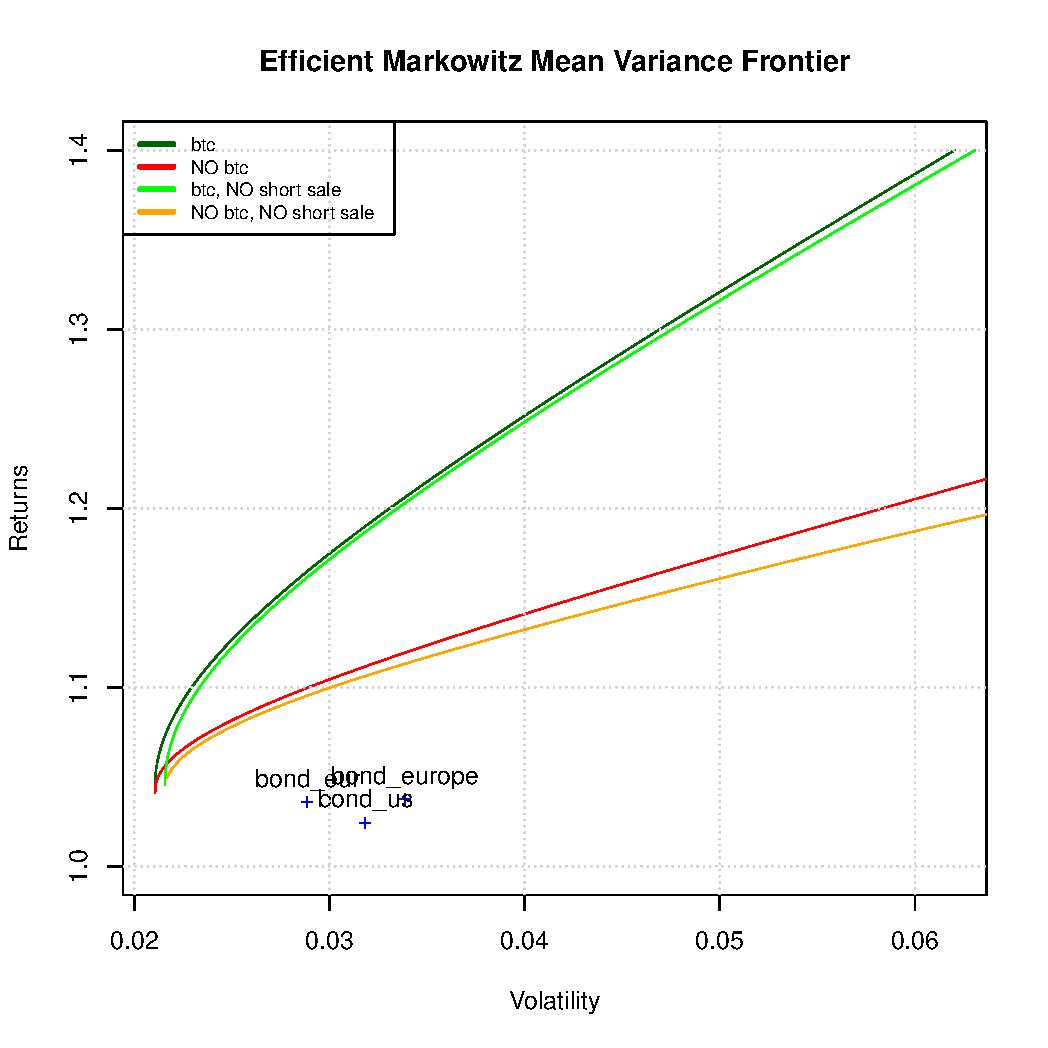
\includegraphics[width=\textwidth]{frontier_markowitz_all_percentage.pdf}
\caption{Plots of the efficient frontier including Bitcoin (green) and without Bitcoin (red,orange). Lighter colours indicate the frontiers where short-selling is not allowed.}
\end{figure}

\begin{figure}[h!]
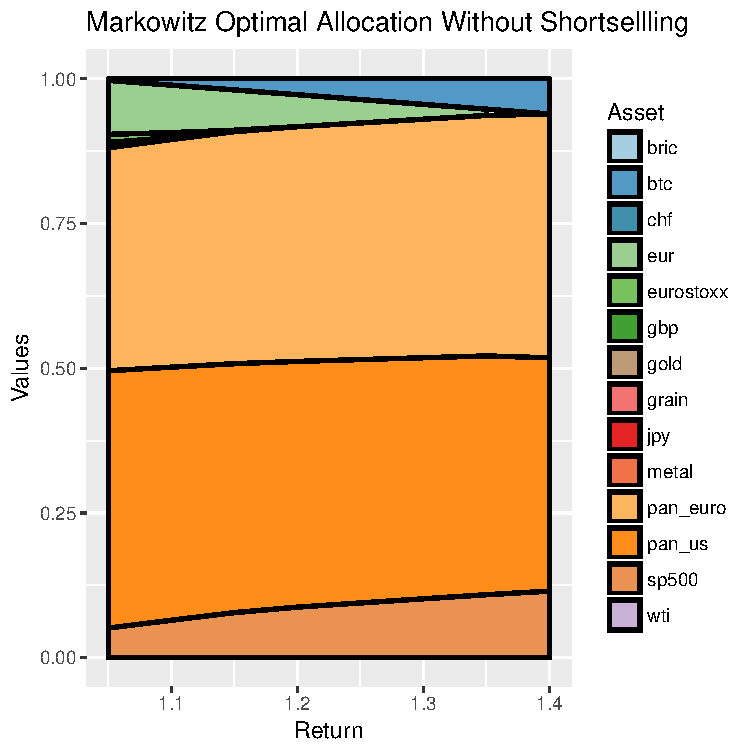
\includegraphics[width=\textwidth]{allocation_markowitz_btc_percentage.pdf}
\caption{Portfolio weights for different values of target return, in the case of no short-selling. Allocation only includes Bitcoin, bond indices and S\&P500.}
\end{figure}





\section{VaR/CVaR Optimization}
Starting from Markowitz original proposal, more and more researchers have studied how to include different risk measures than the variance, since the underlying hypothesis of gaussianity might not be verified.
We decided to consider the \textit{Condition Value at Risk} (CVaR), instead of the simple VaR because of its mathematical properties: CVaR is always a coherent risk measure, while VaR is coherent only under Gaussian Hypothesis.

We gave two implementations of the empirical CVaR. The first is obtained through a kind of bootstrap: considering all given daily return and extracting $n=255$ (vectors of) values from that empirical distribution we can simulate a one-year path of returns. Repeating this process for a given amount of scenarios, we get the empirical distribution of annual returns for all the asset. The portfolio returns are obtained simply by multiplying each scenario return vector by the portfolio weights. 
This approach, though, doesn't take into consideration the actual evolution of the historical returns, but simply draws from a number of previous realizations.
To add some sense of ``history'' we implemented a second slightly different approach.

The second implementation considers the daily returns of the last 5 years and uses them as the realization of $N= 255 * 5 = 1275$ scenarios. From those we compute the daily portfolio returns as before, multiplying by the portfolio weights.

In both cases, we considered the higher $95\%$ set of losses and took the mean to get the empirical CVaR$^{95\%}$.

The mathematical formulation is the following:


\begin{subequations}
\begin{align}
&\!\min_{\mathbf{w}\in \mathbb{R}^{n}}        &\qquad& \text{CVaR}^{95\%}_{ptf}(\mathbf{w}) \\
& \text{subject to} &      & \mathbf{e}'\mathbf{w} = 1 ,\label{eq:constraint1}\\
&                  &      & \mathbf{r}'\mathbf{w} = r_{target},\label{eq:constraint2}\\
&		 &        & w_{i} \geq 0, \text{for} \: i = 1\dots n.
\end{align}
\end{subequations}




\section{Dataset Review}


Besides the time series for Bitcoin, valued as the price of one bitcoin in US dollars, we included in our analysis the following assets, taken from a variety of classes:

\begin{enumerate}
\item Stock indexes:
	\begin{itemize}
		\item S\&P500: American stock market index based on the market capitalization of 500 large company with stock listed either on the NYSE or NASDAQ.
		\item EURO STOXX 50: equity index of eurozone stocks, covering 50 stocks from 11 eurozone countries.
		\item MSCI BRIC: a free float-adjusted index weighted on market capitalization designed to measure the equity market performance across the emerging country indices of Brazil, Russia, India and China.
	\end{itemize}
\item Commodities:
	\begin{itemize}
		\item Gold: price of gold measured in USD/Oz.
		\item WTI: price of crude oil used as benchmark in oil pricing and as the underlying commodity in the NYMEX oil future contracts.
		\item Grain: S\&P GPSCI index that measures the performance of the grain commodity market.
		\item Metals: S\&P GSCI Industrial Metals index that measures the movements of industrial metal prices including aluminium, copper, zinc, nickel and lead.
	\end{itemize}
\item Currencies:
	\begin{itemize}
	\item EUR/USD
	\item GBP/USD
	\item CHF/USD
	\item JPY/USD
	\end{itemize}
\item Bond indexes:
	\begin{itemize}
		\item BBG Pan Euro: Bloomberg Barclays Pan-European Aggregate Index that tracks fixed-rate, investment-grade securities issued in different European currencies.
		\item BBG Pan US: Bloomberg Barclays US Aggregate Bond Index, a benchmark that measures investment grade, US dollar-denominated, fixed-rate taxable bond market.
	\end{itemize}
\end{enumerate}

All data was provided by Bloomberg.

%\begin{itemize}
%\item Bullet point one
%\item Bullet point two
%\end{itemize}

%\begin{enumerate}
%\item Numbered list item one
%\item Numbered list item two
%\end{enumerate}




%% The Appendices part is started with the command \appendix;
%% appendix sections are then done as normal sections
%% \appendix

%% \section{}
%% \label{}

%% References
%%
%% Following citation commands can be used in the body text:
%% Usage of \cite is as follows:
%%   \cite{key}          ==>>  [#]
%%   \cite[chap. 2]{key} ==>>  [#, chap. 2]
%%   \citet{key}         ==>>  Author [#]

%% References with bibTeX database:
\pagebreak
\section{Bibliography}
\bibliographystyle{abbrv}
\bibliography{bitcoin_allocation_bibliography}

%% Authors are advised to submit their bibtex database files. They are
%% requested to list a bibtex style file in the manuscript if they do
%% not want to use model1-num-names.bst.

%% References without bibTeX database:

% \begin{thebibliography}{00}

%% \bibitem must have the following form:
%%   \bibitem{key}...
%%

% \bibitem{}

% \end{thebibliography}


\end{document}

%%
%% End of file `elsarticle-template-1-num.tex'.